\subsection[Prof. Dr. Hilke Brockmann]{Prof. Dr. Hilke Brockmann{\normalfont\normalsize\newline (Joined IUB in August 2006)}}


\vspace{0.3cm}
\textbf{Main Research Interests}\\[-0.25cm]
\begin{enumerate}
\item[$\bullet$]	Social Inequalities, Social Structure
\item[$\bullet$]	Life Course Research, Longitudinal Analysis
\item[$\bullet$]	Population Aging - Its Consequences for Modern States and Societies
\end{enumerate}


\vspace{0.6cm}
\textbf{Research Activities}\\[-0.25cm]

Hilke Brockmann's research in 2006 focused on three research questions: (a) Does population aging increase the demand for health care? (b) How much does a growing older population change the modern state? (c) And how much do policy changes feed back on social inequality? In order to answer the first question Hilke Brockmann conducted a study with colleagues from Universit�t Bremen analyzing health insurance data in order to investigate how health care reforms and health behaviour interact. Two papers have come out of this project so far, one in a peer-reviewed journal. Research concerning the second question is still at an early stage. Hilke Brockmann is currently writing a paper on "Governing generations" in which she compares family, migration and old-age policies in Germany and the US. She also started a small project on the "Demography of Political representatives" and prepared a grant application. Hilke Brockmann is about to finalize two papers one titled "Reforms that go under your skin. Health care and pension policy reform in Germany and the US" the other "Who care when singles die? Families and care at the end of life". Furthermore, a grant application on Health and Families is in preparation.
\begin{figure}[ht]
  \begin{center}
    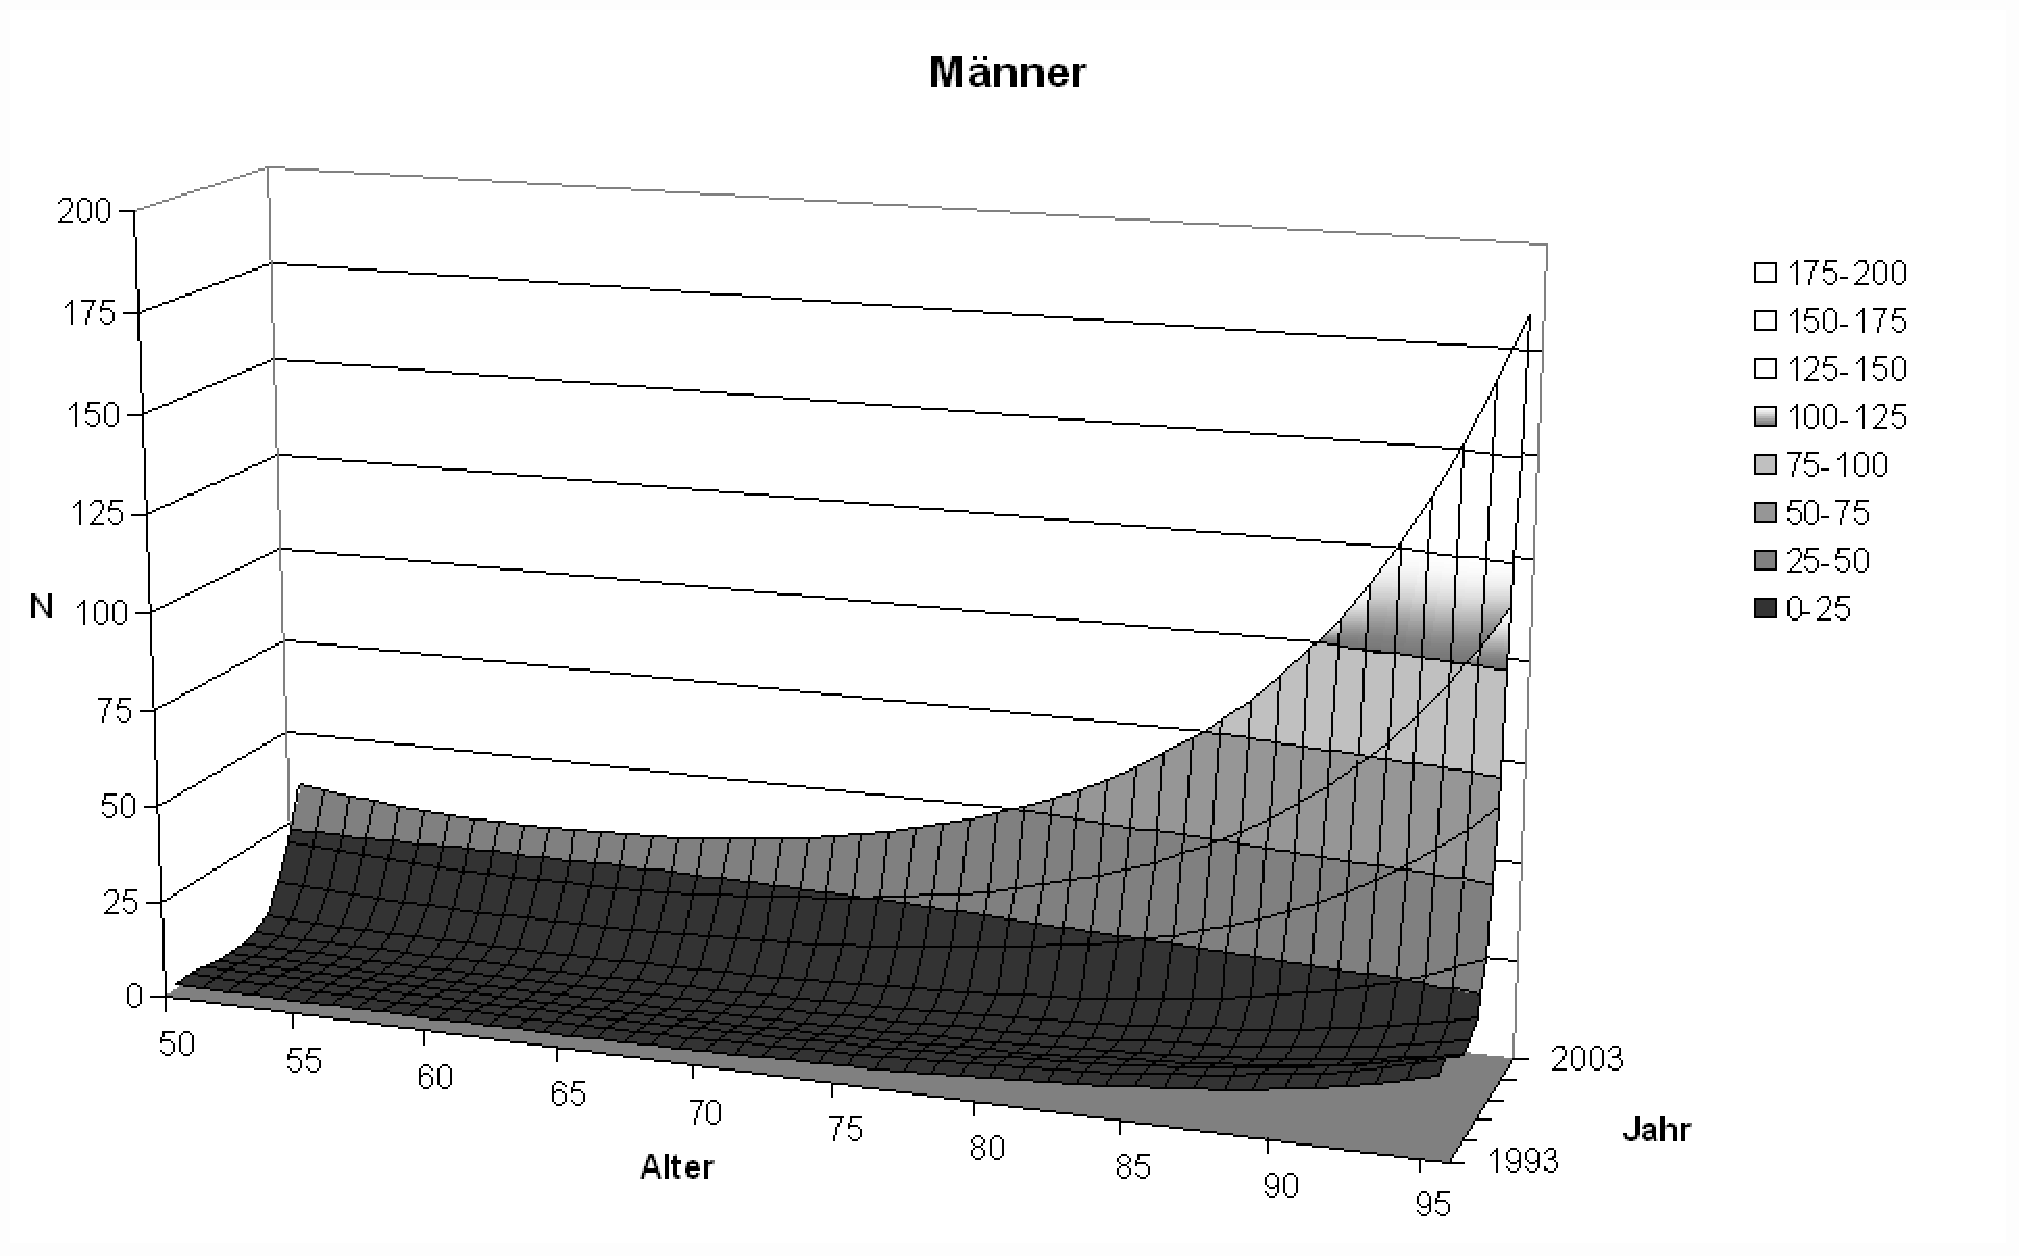
\includegraphics[width=0.95\linewidth]{./SocSci/Brockmann-fig001.pdf}
%   \mycaption{ xxx )}\label{fig:profxxx}
   \end{center}
\end{figure} 
\newpage
\begin{figure}[ht]
  \begin{center}
    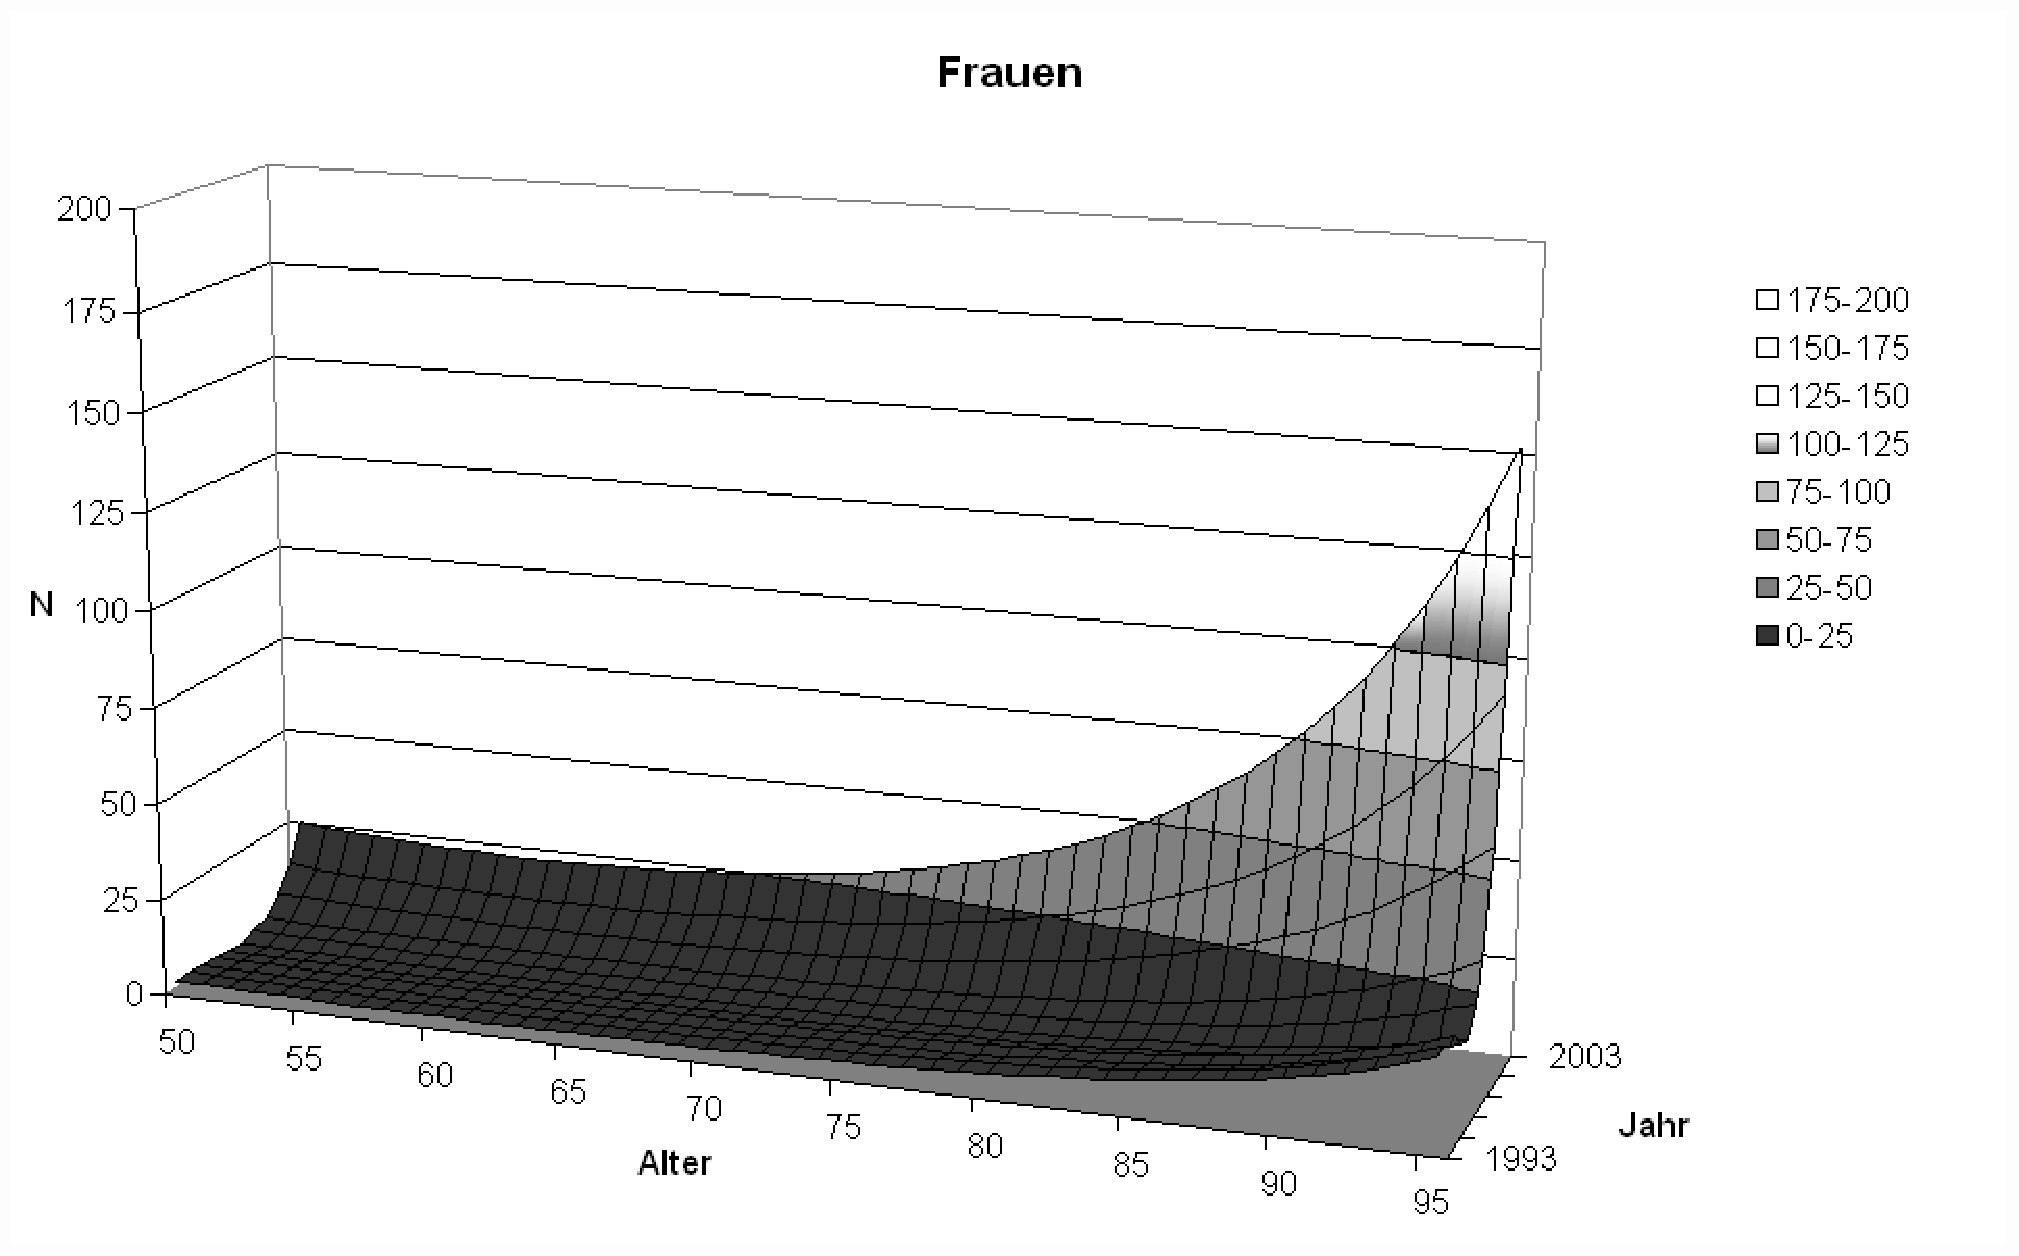
\includegraphics[width=0.95\linewidth]{./SocSci/Brockmann-fig002.pdf}
%   \mycaption{ xxx )}\label{fig:profxxx}
   \end{center}
\end{figure} 

\vspace{0.6cm}
\textbf{Funded Projects}\\[-0.25cm]
\begin{enumerate}
\item[$\bullet$]	Graduate School of Social Sciences (at Universit�t Bremen)
(together with Karin Gottschall, Steffen Mau, and Rainer Baumann),
funded by the VolkswagenStiftung
\end{enumerate}


\vspace{0.6cm}
\textbf{Other Professional Activities}\\[-0.25cm]
\begin{enumerate}
\item[$\bullet$]	Reviews for European Sociological Review
\item[$\bullet$]	Editorial Board of Health Sociology
\end{enumerate}


\vspace{0.6cm}
\textbf{PhD-Students}\\[-0.25cm]

Regine K�ller\newline
\textit{Verrentung = mehr Zeit = mehr Lebensqualit�t? Erwerbst�tigkeit und Zeiterfahrungen im Lebenslauf und die Auswirkungen auf die Gestaltung des Ruhestandes (retirement = more time = more quality of life? The impact of employment and time experience in the life course on the shaping of retirement)}\newline
Defense: March 2006\\[-0.15cm]

Bettina Kohlrausch\newline
\textit{A Ticket to Work? Active Labour Market Policy for the Young Unemployed in Britain and Germany}\\[-0.15cm]

Hao Yuan\newline
\textit{Social Development and Quality of Life: A Comparative Research Between Germany and China}\\[-0.15cm]

Oliver Horrmann\newline
\textit{ "Crowding in" versus "Crowding Out" - about the Impact of Different Welfare States on the Limits and Opportunities of the Provision of Family Care for the Elderly Generation}\\[-0.15cm]


